%%%%%%%%%%%%%%%%%%%%
% DESARROLLO DEL PROYECTO
%%%%%%%%%%%%%%%%%%%%

%\section{Marco de Referencia}
%\subsection{\'Areas Tem\'aticas}
%Listar las \'areas tem\'aticas del proyecto. Para las \'areas propias de la disciplina, utilice las categor\'ias de la ACM. Por ejemplo: D.1.3: Software - Programming Techniques -Concurrent Programming. Ver clasificaci\'on en  (\url{http://www.acm.org/about/class/ccs98-html}). 

\section{Marco Te\'orico}
A continuaci\'on se describen los bases te\'oricas que permiten explicar el contexto de un sistema software de terapia respiratoria requerido:

\subsection{Telemedicina}


La telemedicina es la prestaci\'on de servicios m\'edicos a distancia, para su implementaci\'on se emplean tecnolog\'ias de la informaci\'on. La Organizaci\'on Mundial de la Salud (OMS), declara la Telemedicina como: el suministro de servicios de atenci\'on sanitaria, por profesionales que apelan a las TIC para el intercambio de datos en actividades de diagn\'ostico, tratamiento, prevenci\'on y evaluaci\'on con el fin de mejorar la condici\'on del paciente \cite{19}. La Telemedicina se compone de 4 tipos; Teleconsulta, Teleeducaci\'on, Tele monitoreo y la Telecirug\'ia \cite{20}. Dentro de las ventajas de la telemedicina se encuentran: el acceso e intercambio de informaci\'on m\'edica, el acceso a la prestaci\'on de los servicios de salud, el mejor acompa\~{n}amiento al paciente por parte de los profesionales de salud y la optimizaci\'on de los recursos hospitalarios, entre otros. Actualmente, la incorporaci\'on de dispositivos, servidores de datos basados en la nube a trav\'es de la arquitectura de integraci\'on de la comunicaci\'on (IoT), incorpora dispositivos de bajo costo, bajo consumo energ\'etico y alto rendimiento que facilita el trabajo coordinado de un gran n\'umero de dispositivos que favorece la innovaci\'on en servicios de salud. Gracias a estos avances, emerge la llamada salud m\'ovil (M-Salud) que aprovecha la masificaci\'on del uso de dispositivos m\'oviles de comunicaci\'on como los tel\'efonos celulares y tabletas electr\'onicas para facilitar la interacci\'on entre el paciente y el profesional de la salud en actividades de cuidado de la salud \cite{21}.



\subsection{Covid-19}

En diciembre del 2019 se inici\'o en Wuhan (China) una epidemia de neumon\'ia asociado al coronavirus (SARS-CoV-2), la cual fue declarada como una pandemia por la OMS el 11 de marzo de 2020. La alta mortalidad de la infecci\'on viral est\'a asociada con el desencadenamiento del s\'indrome de dificultad respiratoria aguda el cual est\'a definido por un inicio agudo de edema pulmonar no cardiog\'enico, hipoxemia y la necesidad de ventilaci\'on mec\'anica. Aproximadamente el 30\% de las personas que superan el COVID-19 quedan con insuficiencia de capacidad pulmonar que requiere terapia de re-expansi\'on pulmonar\cite{3}.

\subsection{Inspir\'ometro}

Es un dispositivo m\'edico que se utiliza para ayudar a los pacientes a mejorar el funcionamiento de sus pulmones, conocido tambi\'en como espir\'ometro de incentivo de tratamiento en las terapias respiratorias;  este instrumento mec\'anico ayuda al paciente a mantener el m\'aximo esfuerzo inspiratorio y que consiste en elevar una dos o tres bolas a la parte superior y mantener esa posici\'on. La pelota proporciona retroalimentaci\'on visual para la motivaci\'on, y el dial de flujo se puede ajustar f\'acilmente para aumentar el esfuerzo respiratorio lo cual se condiciona el logro de un esfuerzo inspiratorio m\'aximo mediante esta t\'ecnica que se explica en detalle a continuaci\'on. El uso del inspir\'ometro  requiere que el paciente tenga un adecuado nivel de colaboraci\'on y entendimiento; adem\'as de que su ejecuci\'on debe ser monitoreada y supervisada a fin de asegurar su correcto uso\cite{22}.

\begin{figure}[ht]
\centering
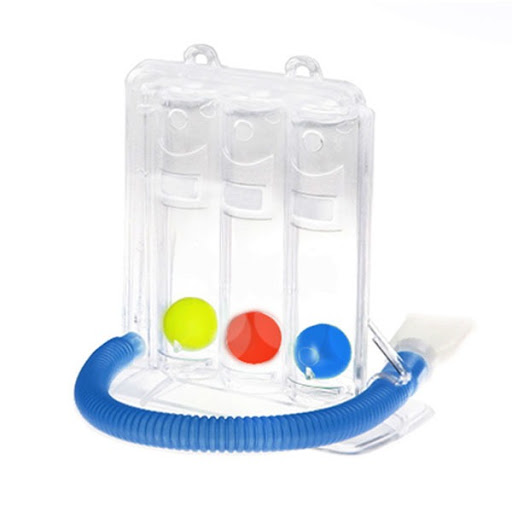
\includegraphics[scale=0.4]{inspiromet.jpg}
\caption{Inspir\'ometro m\'edico.\textit{ LABScI at Stanford }}
\label{1}
\end{figure}
\FloatBarrier



\subsubsection{Incentivo Respiratorio}
 
Un sistema que permite determinar el flujo o el volumen de aire inspirado y brinda informaci\'on al paciente sobre su magnitud.  Entre los beneficios atribuidos a la inspirometr\'ia incentiva se encuentran \cite{23}: a. Aumento de la capacidad inspiratoria, b. Incremento de la presi\'on transpulmonar, c. Fortalecimiento del diafragma y de los m\'usculos intercostales internos, d. Mejoramiento del rendimiento muscular inspiratorio, e. Mejoramiento del mecanismo de la tos,  f. Mejoramiento de la atelectasia al revertirse las \'areas alveolares colapsadas, g. Mejoramiento de la coordinaci\'on neuromuscular, ya que los pacientes pueden conscientemente respirar de manera profunda y lenta, g. Reducci\'on de la hipoxemia al fomentarse una inspiraci\'on profunda, sostenida, lenta y prolongada, lo cual, provoca una presi\'on m\'axima en los alv\'eolos y una inhalaci\'on m\'axima y h.  Mantenimiento de la permeabilidad de las v\'ias a\'ereas m\'as peque\~{n}as. Actualmente, la efectividad de la fisioterapia incentiva depende de una instrucci\'on adecuada al paciente y de la supervisi\'on por parte de un profesional de salud sobre la ejecuci\'on de la terapia respiratoria\cite{24} puesto que no se encuentran disponibles los sistemas incentivos que lleven registro cuantitativo del desempe\~{n}o de la misma.

\subsubsection{Proceso de espirometr\'ia}
Se mide la forma como un paciente inhala o exhala vol\'umenes de aire en funci\'on del tiempo. La inspiraci\'on es el proceso en el cual hay ampliaci\'on de la caja tor\'acica y de los pulmones y as\'i ingresa aire u otra sustancia gaseosa a los pulmones. Los equipos empleados en el monitoreo del flujo de aire tanto en la inspiraci\'on como en la espiraci\'on, utilizan dispositivos para la medici\'on de la variable f\'isica conocidos como transductores de presi\'on. Seg\'un el principio de transducci\'on de presi\'on, los dispositivos empleados para determinar el flujo respiratorio se clasifican en cuatro categor\'ias: neumotac\'ografo, tipo turbina, tipo anem\'ometro y tipo ultras\'onico con diferentes principios de operaci\'on \cite{17}. 


\subsection{Teor\'ia de soluci\'on de problemas inventivos (Triz)}

Un m\'etodo conocido como teor\'ia para resolver problemas de inventiva, esta metodolog\'ia cuenta con un conjunto de herramientas basado en modelos para la generaci\'on de ideas y soluciones innovadoras. Para el dise\~{n}o de un producto centrado en el usuario se considera, ampliar la visi\'on del problema, realizar un an\'alisis sist\'emico del problema, identificar las restricciones de un nuevo producto y ampliar el campo de b\'usqueda de las soluciones \cite{15}.  Dentro de las estrategias que se encuentran en la literatura para el an\'alisis de dise\~{n}o de productos, el uso de la Teor\'ia de Soluci\'on de Problemas Inventivos, TRIZ, es de utilidad en el dise\~{n}o de nuevos productos en un amplio abanico de \'areas incluido el campo de la salud \cite{16}.  Una de las ventajas que presenta TRIZ frente a otras estrategias de ideaci\'on, es su orientaci\'on a la ciencia y la tecnolog\'ia, lo cual permite que la etapa de convergencia de los procesos de dise\~{n}no se pueda realizar de manera \'agil y estructurada. \cite{17} 



\subsubsection{T\'ecnica de las nueve ventanas}

Las nueve ventanas es una t\'ecnica de TRIZ que sirve para visualizar un sistema que desempe\~{n}a una funci\'on principal sobre un producto u objeto, como parte de una estructura jer\'arquica que se desempe\~{n}a en el tiempo y como es su evoluci\'on. Esta forma de an\'alisis sirve para comprender un problema en una forma desagregada e identificar aspectos asociados al problema que no son evidentes desde un an\'alisis funcional. La figura 1.1, muestra el diagrama de las nueve ventanas. En el eje horizontal se representa el tiempo, la parte central el tiempo actual, el pasado a la izquierda y el futuro a la derecha. El eje vertical representa la jerarqu\'ia del problema, el centro es el sistema t\'ecnico que desempe\~{n}a alguna funci\'on, el nivel inferior es su composici\'on o soporte del sistema para que lleve a cabo su funci\'on (el subsistema) y el nivel superior es el contexto donde se encuentra inmerso el sistema (supersistema).\cite{25}

\begin{figure}[ht]
\centering
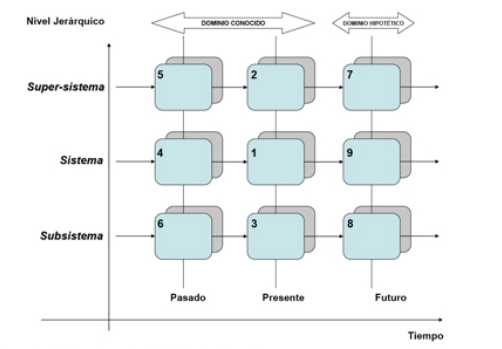
\includegraphics[scale=0.73]{TRIZ.png}
\caption{Diagrama de las nueve ventanas del TRIZ. \textit{Technical Innovation Center Inc.}}
\label{1}
\end{figure}
\FloatBarrier

De manera detallada, en la ventana n\'umero uno se identifica el incentivo respiratorio actual y las variantes actualizadas del mismo, en la ventana dos que el proyecto apoya a los objetivos planteados donde se analiza el panorama de las enfermedades respiratorias como una de las principales causas a nivel mundial no solo por el coronavirus, en la ventana tres se hace la caracterizaci\'on de los componentes de los productos actuales para la rehabilitaci\'on pulmonar, luego se hace un salto hacia el pasado donde se analiza como era los productos pasados para la rehabilitaci\'on respiratoria y cuales han sido sus cambios o mejoras de igual forma en la ventana cinco donde se analiza cuales han sido los factores que han llevado a las enfermedades respiratorias a ser las m\'as mortales a nivel mundial, en la ventana seis a al igual que la ventana tres se hace una caracterizaci\'on de los elementos que conforman el sistema t\'ecnico pasado, luego se hace una mirada hacia el futuro donde la ventana siete se analiza de forma global que deber\'ia existir para que las enfermedades respiratorias disminuyan, en la ventana ocho una descripci\'on de los componentes ideales y finalmente en la ventana nueve se hace una idealizaci\'on de los atributos que deber\'ia tener el producto actual en el futuro.

\subsection{L\'ineas de productos de software (LPS)}

Este software para apoyo a las terapias puede ser m\'as efectivo, si se puede personalizar, es decir, ajustar a las necesidades y caracter\'isticas del paciente. Para el desarrollo de este tipo de sistemas personalizados, se utiliza el paradigma de la Ingenier\'ia de la L\'inea de Productos de Software (ILPS). Este paradigma permite la gesti\'on eficiente de un conjunto de productos que pertenecen a un dominio particular y tienen elementos comunes y variables. Por su parte, una l\'inea de productos de software (LPS) es un conjunto de sistemas de software que comparten componentes reutilizables, satisfacen las necesidades espec\'ificas de un dominio particular y se desarrollan de manera prescrita \cite{14}. Las l\'ineas de productos de software ofrecen una soluci\'on para lograr un equilibrio entre la oferta de productos personalizados y el apoyo a la personalizaci\'on de bajo costo mediante la reutilizaci\'on sistem\'atica de los componentes de software.

\subsection{Gamificaci\'on}

Se define como la aplicaci\'on de elementos y mec\'anicas de juego en entornos ajenos al juego o \textit{non-games activities} que se enfoca en mejorar la experiencia y participaci\'on del usuario con servicios y aplicaciones. Es una t\'ecnica de aprendizaje que traslada la mec\'anica de los juegos al \'ambito educativo-profesional con el fin de mejorar el compromiso y la motivaci\'on para obtener mejores resultados que posteriormente sirven para absorber conocimientos o mejorar alguna habilidad. Las actividades non-games son una forma de entretenimiento que no tiene un ganador o una conclusi\'on real, anteriormente se usaba el termino \"juguete de software\" con el mismo prop\'osito. La principal diferencia entre los videojuegos y los non-games es la falta de metas, objetivos y desaf\'ios estructurados, esto permite al jugador un mayor grado de autoexpresion a trav\'es del juego libre, ya que puede establecer sus propios objetivos para lograrlo.\cite{18}




\subsection{Trabajos Relacionados}

En la literatura es posible encontrar amplia informaci\'on acerca de terapias respiratorias basadas en juegos que se utilizan en los procesos de recuperaci\'on de pacientes y como favorecen su mayor disposici\'on, atenci\'on y vinculaci\'on a un tratamiento. La revisi\'on de patentes de inspir\'ometro, junto con las necesidades de los usuarios, paciente y terapeuta, se convierten en un insumo esencial para el dise\~{n}o de un nuevo producto con el equipo interdisciplinar. 
Para los \'ultimos cinco a\~{n}os se encontraron m\'as de diez patentes asociadas con la inspirometr\'ia, algunas orientadas a la instrumentaci\'on y a la realizaci\'on de la terapia, a continuaci\'on se describen las patentes que aportan a lo objetivos al proyecto. %%


Los dispositivos de espirometr\'ia investigados utilizan la recopilaci\'on de datos para mejorar la eficacia del plan de tratamiento respiratorio. Incluyen una pantalla electr\'onica para proporcionar instrucciones a un paciente y mostrar datos medidos, tambi\'en se realizan una retroalimentaci\'on basada en los datos que se proporciona al paciente para facilitar el cumplimiento de un plan de tratamiento prescrito por el terapeuta respiratorio y tambi\'en se  brinda una estaci\'on de monitoreo. Estas patentes explican la importancia de utlizar  t\'ecnicas de juego en el dispositivo para mantener a los pacientes interesados en realizar sus ejercicios como por ejemplo las alertas autom\'aticas  que recuerdan a los pacientes cu\'ando deben realizar un ejercicio, aprovechando los atributos de los sensores que realizan un seguimiento y detecci\'on paso a paso junto con adaptadores que puede utilizarse como controlador de juego y los ejercicios de respiraci\'on del paciente que se utilizan para realizar ciertas tareas dentro del juego, con ello incentivando a los pacientes a seguir una terapia prescrita y recopilar datos para informar el cumplimiento y la eficacia del tratamiento. \cite{26}

\begin{itemize}
    \item Robert Shane LUTTRELL inventor del Instrumento de terapia respiratoria que ofrece incentivos basados en juegos, capacitaci\'on y recolecci\'on de telemetr\'ia (2019),  incluye un instrumento de terapia respiratoria que proporciona una plataforma de telesalud para el cuidado pulmonar que utiliza sensores de presi\'on adaptados para detectar datos de flujo pulmonar y una placa de circuito adaptada tambi\'en al cuerpo del paciente. La placa de circuito est\'a configurada para transmitir datos, incluidos los datos del flujo pulmonar recopilados, de forma inal\'ambrica a un dispositivo inform\'atico. Los datos de flujo pulmonar recopilados se utilizan en el juego para un incentivo. Dentro del juego, se utilizan comentarios en tiempo real para guiar cada ejercicio. Los videos de entrenamiento incluidos en el juego instruyen al paciente sobre c\'omo configurar y realizar el ejercicio.  Los datos procesados pueden informar a los cuidadores si la patente ha seguido los ejercicios prescritos, as\'i como la calidad (y tendencias) de los ejercicios. Adem\'as, se contempla que los datos recopilados se puedan analizar para detectar tos que pueden ser indicadores de dificultad respiratoria.\cite{26}
    
    \item Dwight Cheu, Michael DiCesare inventores del dispositivo y sistema de terapia respiratoria con capacidades de juego integradas y m\'etodo de uso del mismo; un dispositivo respiratorio basado en procesador para terapia respiratoria que combina juegos y retroalimentaci\'on en tiempo real para guiar al usuario a trav\'es de las t\'ecnicas respiratorias adecuadas. Permite proporcionar una experiencia atractiva, asegurando as\'i que un usuario reciba el m\'aximo beneficio de salud posible de una rutina de terapia respiratoria particular. un dispositivo que se puede conectar a un dispositivo respiratorio existente y proporciona capacidades de gamificaci\'on  para aumentar la tolerancia de un paciente que utiliza el dispositivo y que a su vez crea un m\'etodo de curaci\'on general optimizado. \cite{27}
    
    Un sensor dentro de la c\'amara y acoplado electr\'onicamente al procesador y que comprende una interfaz de comunicaciones acoplada a una red, la interfaz de comunicaciones est\'a configurada para generar una se\~{n}al a una interfaz gr\'afica de usuario basada en el flujo de aire en la c\'amara. en realizaciones opcionales, se puede usar un aceler\'ometro, un giroscopio  o un micr\'ofono. Cada uno de los sensores adicionales puede proporcionar capacidades de juego adicionales que incluyen utilizar la direcci\'on y el movimiento del dispositivo y transmitir ese movimiento a la interfaz para proporcionar capacidad de comunicaci\'on vocal con el juego en s\'i o con otros jugadores.  La capacidad de medir el flujo de aire es importante porque permite que el m\'odulo de evaluaci\'on analice la respiraci\'on de un usuario para determinar su nivel de \'exito en el juego. \cite{27}



\end{itemize}
%revisar
Los anteriores proyectos se enfocan en la capacidad de incentivar a un paciente para realizar una actividad respiratoria utilizando herramientas de hardware y software que se sincronizan entre si, para intercambiar resultados y alcanzar una terapia deseada, sin embargo, estos proyectos no especifican la comunicaci\'on directa entre el dispositivo y el paciente, y como se podr\'ia brindar un acompa\~{n}amiento con un dispositivo para completar una actividad, por lo que los objetivos identificados en las patentes nos permiten diferenciar con los objetivos a desarrollar en este proyecto.







%metodologia

\section{Metodolog\'ia}



Con el fin de dar cumplimiento al objetivo de integrar un sistema software con un dispositivo electr\'onico inspir\'ometro, se desarrollar\'a el software en conjunto con la construcci\'on del dispositivo en la universidad Javeriana. Se cuenta con un equipo interdisciplinar conformado por los profesores expertos en \'areas como software y metodolog\'ias para el an\'alisis de requerimientos, estudiantes de medicina, estudiantes de electr\'onica y de Maestr\'ia en ingenier\'ia de software, dadas las especificaciones del proyecto y el contexto se tiene en cuenta los usuarios, paciente, el terapeuta respiratorio y el profesional de la salud, quienes van a usar el producto con diferentes procedimientos. Este proceso se har\'a en diferentes etapas: \\



\renewcommand{\labelenumii}{\theenumii}
\renewcommand{\theenumii}{\theenumi.\arabic{enumii}.}

\begin{enumerate}
  \item \textbf{Explorar la literatura sobre las pr\'acticas de software relacionadas con un inspir\'ometro y la informaci\'on que se transmite desde el dispositivo, reconocer la etapas de funcionamiento del sistema a desarrollar para llevar a cabo una terapia respiratoria de re-expansi\'on pulmonar.}
  \begin{enumerate}
    \item Recolectar informaci\'on 
    \item Reconocer el funcionamiento del sistema
    \item Analizar los aspectos m\'as importantes sobre los datos que se transmiten desde un sistema remoto
    \item Seleccionar los aspectos importantes sobre el tipo de informaci\'on que se transmite desde un dispositivo inspir\'ometro
    
  \end{enumerate}
  \item \textbf{Definir los requerimientos del sistema mediante la teor\'ia de soluci\'on de problemas inventivos metodolog\'ia TRIZ y la tecnolog\'ia de gamificaci\'on, as\'i como las t\'ecnicas de trabajo e integraci\'on de datos para el sistema software.}
  \begin{enumerate}
    \item Reconocer la informaci\'on que se transmite desde un dispositivo inspir\'ometro
    \item Analizar el estado de la pr\'actica y estudiar directamente el comportamiento del inspir\'ometro
    \item Analizar t\'ecnicas propuestas
    \item Definir los requerimientos utilizando metodolog\'ia TRIZ
  \end{enumerate}
  \item  \textbf{Dise\~{n}ar e implementar un sistema software que se integre con un dispositivo electr\'onico que permita adaptarse al proceso de respiraci\'on de un paciente y que incorpore terapias de re-expansi\'on pulmonar para la recuperaci\'on y mantenimiento de vol\'umenes y capacidades pul-monares.}
  \begin{enumerate}
    \item Dise\~{n}ar el modelo del sistema prototipo
    \item Dise\~{n}ar los componentes del sistema
    \item Dise\~{n}ar las interfaces del sistema
    \item Dise\~{n}o de estrategia de gamificaci\'on
    \item Implementar el modelo propuesto del prototipo
  \end{enumerate}
  \item \textbf{Validar el funcionamiento del software utilizando datos simulados de un paciente con COVID-19 utilizando el inspir\'ometro electr\'onico}
  \begin{enumerate}
    \item Validar las funcionalidades de implementaci\'on
    %\item Proponer casos de pruebas
    %\item Construir casos de pruebas
    %\item Ejecuci\'on de implementaci\'on 
    %\item Realizar simulaciones del c\'odigo
    %\item Realizar las pruebas respectivas propuestas
\end{enumerate}
  
\end{enumerate}




%\section{Resultados Esperados}

%Se ha identificado en la revisi\'on de la literatura que los dispositivos no permiten un registro de datos a partir de una terapia respiratoria, tampoco se especifica un acompa\~{n}amiento remoto en caso de que el sistema no tenga un acceso a una red estable. Se contar\'a con una metodolog\'ia que permita identificar los requerimientos del sistema bajo las posibles soluciones identificadas y potencialmente usar una t\'ecnica de gamificaci\'on en un software que permite hacer el registro de los datos que se solicitan y que pueda tener un funcionamiento offline.  


\section{Recursos a Emplear}
\subsection{Humanos}
La estimaci\'on de recursos humanos se calcul\'o con base en la dedicaci\'on de tiempo requerida para el proyecto y el valor de la hora de trabajo en el mismo, obteniendo los datos que se presentan en las siguientes subsecciones.

\subsubsection{Director}

\begin{table}[ht]
\centering
\begin{tabular}{|l|l|l|}
\hline
\textbf{Dedicaci\'on}      & \textbf{Valor Hora} & \textbf{Total} \\ \hline
2 Horas/semana x 8 meses & \$70.000            & 4.480.00       \\ \hline
\end{tabular}
\end{table}

\subsubsection{Estudiante}

\begin{table}[ht]
\centering
\begin{tabular}{|l|l|l|}
\hline
\textbf{Dedicaci\'on}       & \textbf{Valor Hora} & \textbf{Total} \\ \hline
12 Horas/semana x 8 meses & \$ 45.000           & \$ 17.280.000  \\ \hline
\end{tabular}
\end{table}


\subsection{Otros Recursos}

\begin{table}[ht]
\centering
\begin{tabular}{|l|l|}
\hline
\textbf{Rubro}        & \textbf{Total} \\ \hline
Equipos de computo    & \$2.000.000   \\ \hline
Software              & \$1.000.000    \\ \hline
Bibliograf\'ia          & \$200.000    \\ \hline
Recursos Electr\'onicos & \$1.000.000    \\ \hline
\textbf{Total}        & \$15.000.000   \\ \hline
\end{tabular}
\end{table}





\newpage

\section{Cronograma}

Para el desarrollo del proyecto se plantearon las siguientes actividades de tal manera que se pudiera lograr el objetivo del mismo. Las actividades est\'an definidas para realizarse en 6 meses lo cual se represent\'o en 24 semanas donde se trabajara 5 d\'ias por semana. La distribuci\'on  se muestra a continuaci\'on.
%en los cuadros \ref{t1}, \ref{t2}, \ref{t3}, \ref{t4} y \ref{t5}.


%GANT 1--------------------------------

\begin{figure}[ht]
\centering
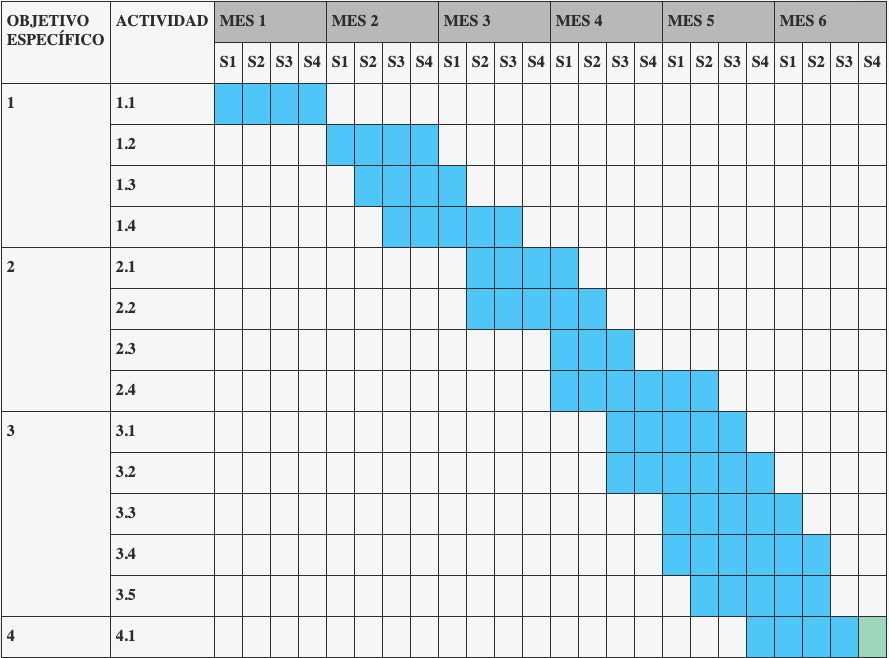
\includegraphics[scale=0.5]{gant.png}
%\caption{Diagrama de las nueve ventanas del TRIZ. \textit{Technical Innovation Center Inc.}}
%\label{1}
\end{figure}
\FloatBarrier

 



    





